%\documentclass[a4paper,svgnames,10pt]{book}
\documentclass[10pt,A4]{article}

\usepackage[utf8x]{inputenc}
%\usepackage{tikz}
\usepackage{varwidth}
\usepackage{linegoal}
\usepackage[explicit]{titlesec}
%\usepackage[margin=1.5cm]{geometry}
\usepackage{lipsum}

%star rating system
\usepackage{tikz}
\usetikzlibrary{shapes.geometric}
\newcommand\score[2]{
\pgfmathsetmacro\pgfxa{#1+1}
\tikzstyle{scorestars}=[star, star points=5, star point ratio=2.25, draw, inner sep=1.3pt, anchor=outer point 3]
  \begin{tikzpicture}[baseline]
    \foreach \i in {1,...,#2} {
    \pgfmathparse{(\i<=#1?"orange":"white")}
    \edef\starcolor{\pgfmathresult}
    \draw (\i*1.75ex,0) node[name=star\i,scorestars,fill=\starcolor]  {};
   }
  \end{tikzpicture}
}
%wheel rating system
\newcommand\wheelrate[2]{
\pgfmathsetmacro\pgfxa{#1}
  \begin{tikzpicture}[baseline=-1.5mm]
    \foreach \i in {1,...,#2} {
    \pgfmathparse{(\i<=#1?"wheel-on":"wheel-off")}
    \edef\imgname{\pgfmathresult}
    \draw (\i*2.25ex,0) node[inner sep=0pt] (whitehead)
        {\includegraphics[height=3mm]{\imgname}};
    }
  \end{tikzpicture}
}
%
% arrow
\usetikzlibrary{fadings,shadows,shapes.arrows}
%
\tikzfading[
  name=arrowfading,
  top color=transparent!0,
  bottom color=transparent!95
]
\newcommand*{\tikzarrow}[2]{%
  \tikz[
    baseline=(A.base),             % Set baseline to the baseline of node content
    font=\footnotesize\sffamily    % Set fontsize of the node content
  ]
  \node[
    single arrow,                  % Shape of the node
    single arrow head extend=4pt,  % Actual width of arrow head
    single arrow tip angle=150,    % Adjust arrow tip angle
    shape border rotate=270,       % Rotate the arrow shape to point down
    draw=black!25,                   % Draw the node shape (with certain border color
    inner sep=2pt,                 % Separation between node content and node shape
    top color=white,               % Shading color on top of node
    bottom color=#1,               % Shading color on bottom of node
    general shadow={               % Specifications for the shadow
      fill=black,
      shadow yshift=-0.5ex,
      path fading=arrowfading
    }
  ] (A) {#2};%
}

%for cell's color of table
\usepackage{xcolor,colortbl}

%for images
\usepackage{graphicx}
\graphicspath{ {./images/} }

%set margin
\usepackage[a4paper]{geometry}		
\geometry{top=1cm, bottom=-.6cm, left=0.4cm, right=1cm} 

\newcolumntype{P}[1]{>{\centering\arraybackslash}p{#1}}

\definecolor{myblue}{RGB}{158,158,255}

\titleformat{name=\section,numberless}
  {\normalfont\Large\bfseries}{}{0em}
  {%
  \begin{tikzpicture}
  \node[inner xsep=0pt,text width=\textwidth,
    align=left,left color=myblue,right color=myblue!10] 
    {\parbox[t]{\linewidth}{\raggedright#1}};
  \end{tikzpicture}%
  }

\begin{document}
%
\begin{minipage}[c]{0.2\textwidth}
\vspace{-5mm}
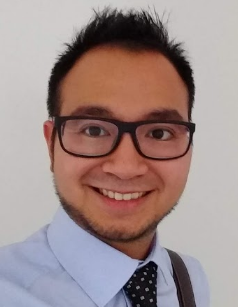
\includegraphics[width=30mm]{myphoto}
\end{minipage}
\begin{minipage}[c]{0.3\textwidth}
\textsc{\large \bf Minh Quan NGUYEN}\\
\textcolor{blue}{\large \bf DevOps Solution Architect }\vspace{5pt}\\
8+ yrs of exp, 33 yr-old\\
+33 6 10 87 32 30\\
%\textcolor{blue}{\underline{\bf nguyen.ensma@gmail.com}}\\
\textcolor{blue}{\bf nguyen.ensma@gmail.com}\\
3 rue des bouquetins\\
31200 Toulouse\\
Nationality: French \& Vietnamese\\
Driving license: B\\
\end{minipage}
\begin{minipage}[c]{0.5\textwidth}
\begin{tabular}{|P{0.4\textwidth}P{0.4\textwidth}|}
\hline
\vspace{5mm} & \vspace{5mm}\\
My Django Web App \newline \tikzarrow{gray}{QR SCAN} & My DevOps git repo \newline \tikzarrow{gray}{QR SCAN}\\

\includegraphics[width=30mm]{antiphotomaton-webapp} & 
\includegraphics[width=30mm]{devopsEcoSystem-git}\\
\hline
\end{tabular}
\end{minipage}
%---------------------------------------------------------------------------------------
%	ABOUT ME
%----------------------------------------------------------------------------------------
%
\textcolor{black}{\large \bf About me\\}
\noindent\textcolor{blue!10}{\rule{\textwidth}{.8mm}}
\begin{quotation}
"Administrator of a DevOps Platform in Kubernetes and having set up a whole Platform as a Service from scratch in a big digital transformation project are the cutting edge knowledge \& experience that I want to contribute to your team. 
Please dont hesitate to contact me to discuss about our future collaboration!"
\end{quotation}
\begin{minipage}[c]{0.7\textwidth}
%
%---------------------------------------------------------------------------------------
%	EXPERIENCE
%---------------------------------------------------------------------------------------
\section*{\hspace{0.5cm}Professional experience}
%
\begin{tabular}{p{2cm}p{11cm}}
\multicolumn{2}{l}{\textcolor{black}{\bf Capgemini DEMS / St Martin Touch}}\\
\noindent\textcolor{blue}{\rule{\textwidth}{.8mm}}\\
%
\textcolor{black}{\bf 2019 - Now} & \textcolor{black}{\bf DevOps PaaS Administrator}
\begin{itemize}
  \item \small Developed a DevOps Platform on premise cloud using Kubernetes
  \item \small Develop Demonstrators for DevOps technologies \& tools   
  \item \small Establish DevOps guides and best pratices for dev teams
  \item \small Provide supports on migration \& integration into new platform
\end{itemize}\\
%
\multicolumn{2}{l}{\textcolor{black}{\bf Altran Technologies / Blagnac}}\\
\noindent\textcolor{blue}{\rule{\textwidth}{.8mm}}\\
%
\textcolor{black}{\bf 2017 - 2018} & \textcolor{black}{\bf Scientific software development engineer}
\begin{itemize}
  \item \small Developed \& calibrate a simulator predicting the airgap between rotor and stator of turbo reactor
  \item \small Optimized the algorithm to speed up the calculation
\end{itemize}\\
%
\textcolor{black}{\bf 2013 - 2017} & \textcolor{black}{\bf Multiphysics \& PLM software development engineer}
\begin{itemize}
  \item \small Developed APIs enabling the data exchange between two simulation software under the european R\&D project TOICA
  \item \small Partipated in the development of a demonstrator of the co-simulation capacity
\end{itemize}\\
%
\textcolor{black}{\bf 2012 - 2013} & \textcolor{black}{\bf Aerodynamics simulation platform administrator}
\begin{itemize}
  \item \small Provided supports for end-users of the simulation tools.
  \item \small Renewed \& translated tools from out-of-date technologies to the new one
\end{itemize}
%
\end{tabular}
%
%---------------------------------------------------------------------------------------
%	EDUCATION
%---------------------------------------------------------------------------------------
\vspace*{-8mm}
\section*{\hspace{0.5cm}Diploma \& Certificates}
%
\begin{tabular}{P{2cm}p{11cm}}
\textcolor{black}{\bf 2019} & \textcolor{black}{ \bf Certificate - SAFe for team}  \newline \small \textcolor{gray}{Scaled Agile} \\
\textcolor{black}{\bf 2019} & \textcolor{black}{ \bf Certificate - Marlogic Database fundamentals} \newline \small \textcolor{gray}{MarkLogic training course} \\
\textcolor{black}{\bf 2018} & \textcolor{black}{ \bf Certificate - Architecting Smart IoT devices} \newline \small \textcolor{gray}{Coursera EIT Digital} \\
\textcolor{black}{\bf 2016} & \textcolor{black}{ \bf Certificate - Agile \& Scrum method} \newline \small \textcolor{gray}{Actinuum SARL} \\
\textcolor{black}{\bf 2015} & \textcolor{black}{ \bf Certificate - Module ECS in NX software} \newline \small \textcolor{gray}{Seimens Industry Software SAS} \\
\textcolor{black}{\bf 2011} & \textcolor{black}{ \bf French Diplôme d'Ingénieur} \newline \small \textcolor{gray}{ISAE-ENSMA (major de promo)} \\
\end{tabular}
%
%---------------------------------------------------------------------------------------
%	LANGUAGES
%---------------------------------------------------------------------------------------
%\section*{\hspace{0.5cm}Languages}
\end{minipage}
\begin{minipage}[t]{0.01\textwidth}
\hspace{1mm}
\end{minipage}
\begin{minipage}[c]{0.25\textwidth}
%
%---------------------------------------------------------------------------------------
%	COMPETENCES
%---------------------------------------------------------------------------------------
\begin{tabular}{|lc|}
\hline
\multicolumn{2}{|c|}{\cellcolor{white} \bf DevOps Infrastructure} \\
\hline
Docker & \wheelrate{5}{5} \\
Kubernetes & \wheelrate{4}{5} \\
Rancher & \wheelrate{5}{5} \\
Helm & \wheelrate{4}{5} \\
AWS & \wheelrate{3}{5} \\
Openshift & \wheelrate{2}{5} \\
\hline
\multicolumn{2}{c}{} \\
\hline
\multicolumn{2}{|c|}{\cellcolor{white} \bf DevOps Components} \\
\hline
Git & \wheelrate{5}{5} \\
Jenkins & \wheelrate{5}{5} \\
Artifactory & \wheelrate{5}{5} \\
Sonarqube & \wheelrate{4}{5} \\
Ansible & \wheelrate{3}{5} \\
\hline
\multicolumn{2}{c}{} \\
\hline
\multicolumn{2}{|c|}{\cellcolor{white} \bf Front end} \\
\hline
Angular & \wheelrate{3}{5} \\
Djanggo & \wheelrate{3}{5} \\
React & \wheelrate{2}{5} \\
HTML & \wheelrate{4}{5} \\
CSS & \wheelrate{4}{5} \\
\hline
\multicolumn{2}{c}{} \\
\hline
\multicolumn{2}{|c|}{\cellcolor{white} \bf Back end} \\
\hline
Python & \wheelrate{5}{5} \\
VB.NET & \wheelrate{5}{5} \\
Java & \wheelrate{4}{5} \\
C++ & \wheelrate{4}{5} \\
Node.js & \wheelrate{3}{5} \\
\hline
\multicolumn{2}{c}{} \\
\hline
\multicolumn{2}{|c|}{\cellcolor{white} \bf Database} \\
\hline
mySQL & \wheelrate{4}{5} \\
Marklogic & \wheelrate{3}{5} \\
MongoDB & \wheelrate{3}{5} \\
\hline
\multicolumn{2}{c}{} \\
\hline
\multicolumn{2}{|c|}{\cellcolor{white} \bf Project Manangement Tools} \\
\hline
version One & \wheelrate{4}{5} \\
Trello & \wheelrate{5}{5} \\
GANTT Chart & \wheelrate{4}{5} \\
\hline
\multicolumn{2}{c}{} \\
\hline
\multicolumn{2}{|c|}{\cellcolor{white} \bf Scientific Simulation Software} \\
\hline
NX/TMG & \wheelrate{5}{5} \\
Ansys & \wheelrate{3}{5} \\
AMESim & \wheelrate{4}{5} \\
\hline
\multicolumn{2}{c}{} \\
\hline
\multicolumn{2}{|c|}{\cellcolor{white} \bf Languages} \\
\hline
Vietnamese & \wheelrate{5}{5} \\
English & \wheelrate{5}{5} \\
French & \wheelrate{5}{5} \\
Spanish & \wheelrate{2}{5} \\
\hline
\end{tabular}
%
\end{minipage}
%
\end{document}